\chapter{A Arquitetura da Solução} 

Para sanar o gargalo operacional imposto pela extração manual de dados não estruturados, foi concebida uma arquitetura baseada em eventos lógicos e armazenamento em nuvem. Este capítulo descreve conceitualmente o novo fluxo de informações da Veeries, detalhando o ambiente de execução, o ciclo de vida dos arquivos e a transição da granularidade dos dados através das camadas do \textit{pipeline}.

\section{Ambiente de Execução e Orquestração}

A infraestrutura de armazenamento do projeto foi estabelecida sobre o ecossistema de nuvem sincronizada da organização (utilizando as plataformas \textit{OneDrive/SharePoint}). Essa escolha garante alta disponibilidade e espelhamento nativo dos arquivos do \textit{pipeline} com as estações de trabalho da equipe.

Como as fontes externas não possuem uma data de publicação exata ou previsível para a emissão dos seus relatórios mensais em PDF, a adoção de um agendador de tarefas tradicional (baseado em tempo cronometrado) resultaria em execuções ociosas ou falhas por ausência de arquivos. Portanto, o acionamento do \textit{pipeline} baseia-se em uma arquitetura orientada a eventos, com orquestração sob demanda. 

O fluxo se inicia quando o analista responsável pelo monitoramento recebe o documento da fonte (via e-mail ou portais do mercado). O arquivo é então salvo de maneira padronizada no diretório de entrada inicial do \textit{pipeline} (denominado \texttt{01\_RAW}). Após o armazenamento, o usuário aciona a execução do processamento através de um \textit{bot} no aplicativo de mensagens \textit{Telegram}, o qual atua como o gatilho externo. Este \textit{bot} envia um comando (via \textit{webhook} ou requisição de API) que inicia a rotina de execução do repositório no \textit{GitHub}, transferindo o processamento pesado para o ambiente em nuvem da aplicação.

A \autoref{fig_arquitetura} ilustra o diagrama esquemático deste fluxo lógico, desde a captura dos dados crus até a sua disponibilização para os usuários analistas de mercado.

\begin{figure}[htb]
    \caption{\label{fig_arquitetura}Diagrama de Arquitetura do \textit{Pipeline Medallion}}
    \begin{center}
        % DICA: Substitua 'Example.png' pelo nome exato do seu arquivo de imagem na pasta 'imagens'
        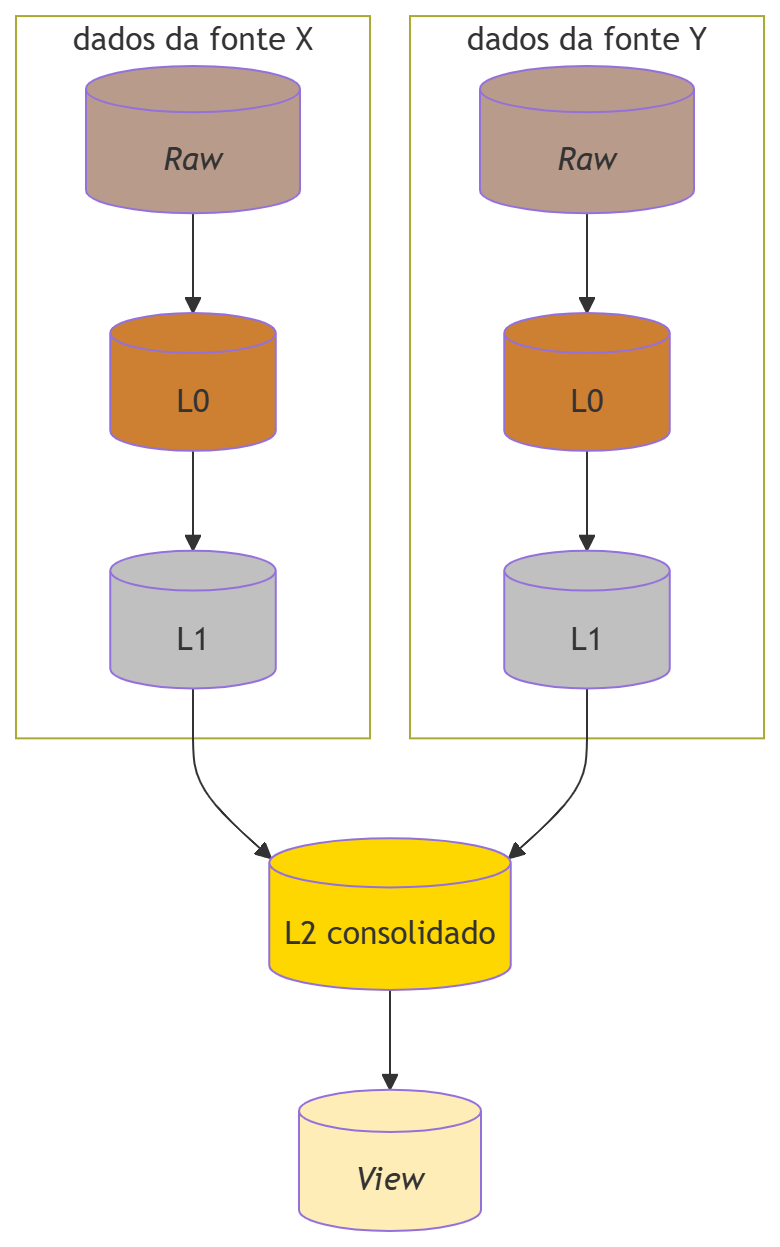
\includegraphics[scale=0.3]{imagens/arquitetura.png}
    \end{center}
    \legend{Fonte: Elaborado pelo autor.}
\end{figure}

\section{Fluxo e Evolução Estrutural dos Arquivos}

Uma diretriz central desta arquitetura foi o isolamento contínuo das fontes de dados durante as etapas de limpeza e validação, a fim de evitar que anomalias em um relatório comprometessem a ingestão do outro. A \autoref{fig_fluxo} detalha visualmente as etapas de processamento e a evolução estrutural dos arquivos dentro do \textit{pipeline}.

\begin{figure}[htb]
    \caption{\label{fig_fluxo}Fluxo de Processamento de Dados entre as Camadas}
    \begin{center}
        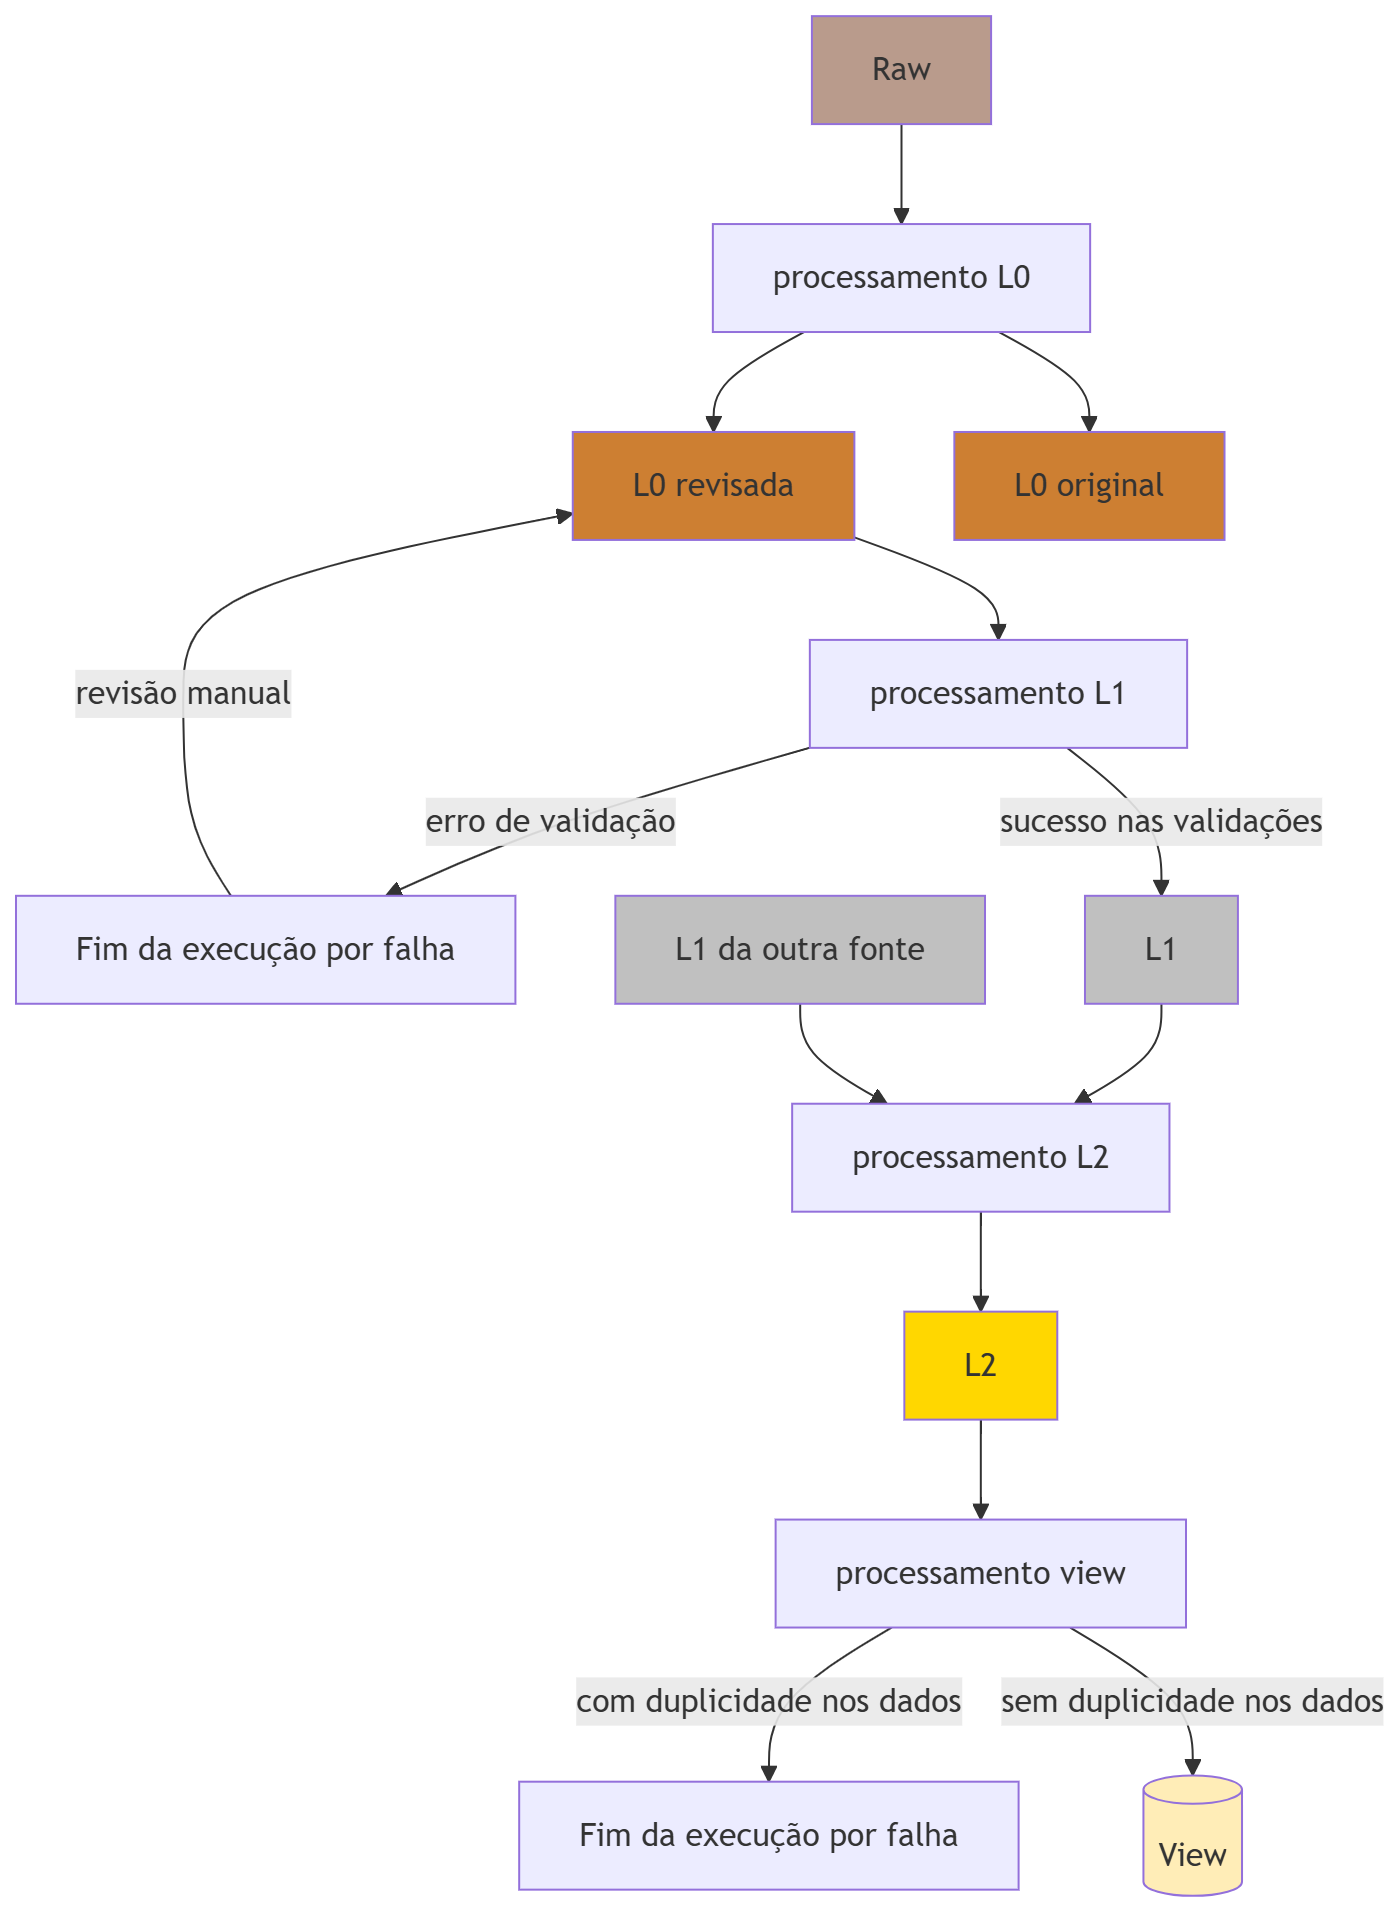
\includegraphics[scale=0.25]{imagens/fluxo_processamento.png}
    \end{center}
    \legend{Fonte: Elaborado pelo autor.}
\end{figure}

A transição e consolidação da informação ocorrem de maneira gradativa através das camadas:

\begin{itemize}
    \item \textbf{Camada \textit{Raw} (Crua):} Os arquivos que ingressam nesta camada preservam seu formato nativo (PDF). A granularidade é estritamente unitária: cada arquivo corresponde a um documento em PDF de uma única fonte de informação, retratando uma única data de emissão e um mês de referência específico. Os arquivos são mantidos em diretórios separados por fonte.
    
    \item \textbf{Camada \textit{Bronze} (L0 Original e Revisada):} Após o acionamento do \textit{parser}, o dado é convertido do formato PDF para arquivos tabulares (arquivos .CSV), preservando a granularidade original. Assim, na camada L0, cada CSV gerado continua representando os dados de uma única fonte para uma referência temporal específica. A fragmentação da L0 permite a tolerância a falhas na extração do texto antes de avançar para as validações estruturais.
    
    \item \textbf{Camada \textit{Silver} (L1):} A transição para a camada L1 engloba a imposição de esquemas e a validação matemática. A granularidade do arquivo sofre sua primeira alteração arquitetural: o arquivo gerado na camada L1 passa a representar a união consolidada de todos os arquivos históricos extraídos da L0 Revisada. Contudo, essa consolidação ainda ocorre de maneira particionada por fonte de informação. Isso garante que qualquer falha de validação ou processamento em uma das origens possa ser identificada e isolada sem interferir na disponibilidade dos dados da outra fonte.
    
    \item \textbf{Camada \textit{Gold} (L2):} É na penúltima camada de processamento que ocorre a consolidação global do \textit{pipeline}. Os dados validados das diferentes origens (Fonte X e Fonte Y) convergem para formar um único documento mestre de \textit{data warehouse}. A granularidade torna-se abrangente e multiorigem. 
\end{itemize}